\documentclass[]{article}
\usepackage{packages}
\usepackage{verbatim}

\usepackage{biblatex}
\addbibresource{bibliography.bib}

\newcommand{\ve}[1]{\mathbf{#1}}
\newcommand{\ham}{\mathcal{H}}
\newcommand{\ket}[1]{\left| #1 \right\rangle}
\newcommand{\bra}[1]{\left\langle #1 \right|}
\newcommand{\bracket}[2]{\left\langle #1 | #2 \right\rangle}
\newcommand{\bracketop}[3]{\left\langle #1 |#3| #2 \right\rangle}

\begin{document}

\begin{titlepage}
    \vfill
    \begin{figure}[h]
        \centering
        \includegraphics[width=8cm]{./images/unitnlogo.png}
        \label{fig:logo}
    \end{figure}
    \vspace{5pt}
    \centerline{\itshape\huge University of Trento, Department of Physics}
    \vspace{10pt}
    \centerline{\emph{\huge Bachelor Degree in Physics}}
    \vspace{100pt}
    \centerline{\bfseries\Huge Negative absolute temperatures}
    \vspace{100pt}
    \centerline{\Large \hspace{100pt} \textit{Candidate:} Matteo Zortea
    \hspace{50pt} \textit{Supervisor:} Raffaello Potestio \hspace{100pt}}
    \vfill
\end{titlepage}

\hypersetup{linkcolor=black}
\tableofcontents
\newpage
\hypersetup{linkcolor=cyan}

\section*{Introduction}
Everyone has an intuitive idea of what temperature is in everyday's life, for example as a quantity that provides us information 
about the environment. \\ 
Temperature is measured everyday via thermometers, particular devices that provide a number that quantifies the grade of \emph{hotness} of what we are observing. \\
An adequate measure of temperature is given by a number and a physical unit. All the thermometers give the same number when used to measure the temperature of the same object, provided that 
the number is expressed always in the same physical unit. The most common temperature unit is the degree Celsius: this scale of values is normally estabilished by fixing the values of temperature of two well known
physical phenomena and assuming a linear relation between temperature and the physical property of the material used as a thermometer, may it be the height of a liquid column in a bulb or an elastic deformation of a certain solid material.
A roughly good calibration of a thermometer in the Celsius scale can be done by assigning a thermometer a value of $0^\circ$C) (0 degrees Celsius) at the frozen point of water, and $100^\circ$C at the boiling point of water. A more sophisticated and precise way to calibrate a thermometer 
on the Celsius scale consists in assigning the value of $-273.15^\circ$C to the \emph{coldest} temperature admitted according to nowadays' physics, and $0.01^\circ$ C to the triple point of whater, that 
is the precise situation in which water coexists in liquid, solid and gaseous form. \\
Another interesting temperature scale is the one measured in degrees Kelvin (K), called the \emph{absolute temperature}. This scale of temperature is 
defined in a way such that it gives a values of $0$ K at the coldest possible situation admitted by physics, the so called \emph{absolute zero} point: this means that no physical systems can be cooled more than a system 
whose absolute temperature is $0$ K. \\
The purpose of this thesis is to introduce the concept of \emph{negative absolute temperatures}. This does not constitutes a contradiction to what told before because negative absolute temperatures should not be searched below the absolute zero, but rather 
below infinity: negative absolute temperatures are hotter that all the positive temperatures. The world of negative absolute temperatures is often accompanied by strange phenomena: for example, in this range of temperatures,
a cooler body get cooled down spontaneously giving heat to a hotter body, increasing the temperature of the latter. \par
\vspace{10pt}
In the first chapter of this thesis I will first introduce the concept of temperature in a rigorous way, according to physical laws, justifying the existence of negative absolute temperatures basing on thermodynamical arguments. \\
A simple system that admits negative temperatures will then be presented in chapter \ref{sec:TLS}, namely the two level system. \\
In chapter \ref{sec:PandP} I will then show that negative absolute temperatures were experimentally observed by Purcell and Pound in 1950. 
After that discovery, some criticisms were moved against the definition of the entropy used the define the absolute scale, putting in doubt the existence of negative temperatures: this will be discussed in chapter \ref{sec:entropy}. \\
Finally a simulation of a system at negative temperature will be presented in the last chapter.

\newpage

\section{Formal definition of temperature}
\label{sec:temperature}
\subsubsection*{Thermal equilibrium}
Definition of macroscopic variables, equilibrium
\subsubsection*{Temperature as equivalence class with respect to equilibrium equivalence relation}
Let us consider three systems $A, B, C$ whose equilibrium properties are described by the variables
$\{X_1, X_2, \dots\}$, $\{Y_1, Y_2, \dots\}$ and $\{Z_1, Z_2, \dots\}$. \\
If $A$ and $B$ are in equilibrium for some values $\{X_1, X_2, \dots\}$ and $\{Y_1, Y_2, \dots\}$ of the coordinates, then there must be a relation between $\{X_1, X_2, \dots\}$ and $\{Y_1, Y_2, \dots\}$ which can be expressed as
\begin{equation*}
    f_{AB}(X_1, X_2, \dots, Y_1, Y_2, \dots) = 0
\end{equation*}
In an analogous manner, if $B$ and $C$ are in equilibrium for some values $\{Y_1', Y_2', \dots\}$ and $\{Z_1, Z_2, \dots\}$ of the coordinates, then there must be a constrain on the values $\{Y_1', Y_2', \dots\}$ and $\{Z_1, Z_2, \dots\}$, which we express as
\begin{equation*}
    f_{BC}(Y_1', Y_2', \dots, Z_1, Z_2, \dots) = 0
\end{equation*}
The equations above can be inverted to espress one thermodynamic coordinate as a function of the others, or in other words, the above expressions may be written as
\begin{gather*}
    Y_1 = g_{AB} (X_1, X_2, \dots, Y_2, \dots) \\
    Y_1' = g_{BC} (Y_2', \dots, Z_1, Z_2, \dots)
\end{gather*}
Now let us bring the system $B$ in the same state in both cases, which means imposing $Y_1 = Y_1'$ and $Y_2 = Y_2'$. The last two equations implies that 
\begin{equation}
    g_{AB} (X_1, X_2, \dots, Y_2, \dots) = g_{BC} (Y_2, \dots, Z_1, Z_2, \dots)
    \label{eq:equality_of_g}
\end{equation}
or
\begin{equation*}
    G_{ABC} (X_1, X_2, \dots, Y_2, \dots, Z_1, Z_2, \dots) = 0
\end{equation*}
One can use this relation to express $X_1$ as 
\begin{equation}
    X_1 = h_{ABC}(X_2, \dots, Y_2, \dots, Z_1, Z_2)
    \label{eq:X1_equilibrium_ABC}
\end{equation}
According to the zeroth principle of thermodynamics, which states that if $A$ and $B$ are in equilibrium and $B$ and $C$ are in equilibrium then $A$ and $C$ are in equilibrium 
\footnote{or, alternatively, that equilibrium is an equivalence relation}, then
there must be a constrain on the values ${X_1, X_2, \dots}$, ${Z_1, Z_2, \dots}$ which can be expressed as 
\begin{equation*}
    f_{AC} (X_1, X_2, \dots, Z_1, Z_2, \dots) = 0
\end{equation*}
which means that $X_1$ can be expressed as
\begin{equation}
    X_1 = g_{AC} (X_2, \dots, Z_1, Z_2, \dots)
    \label{eq:X1_equilibrium_AC}
\end{equation}
imposing the equality between \ref{eq:X1_equilibrium_ABC} and \ref{eq:X1_equilibrium_AC}
\begin{equation*}
    g_{AC} (X_2, \dots, Z_1, Z_2, \dots) = h_{ABC}(X_2, \dots, Y_2, \dots, Z_1, Z_2)
\end{equation*}
The term on the lefts does not depend on the coordinates of $B$. This means that both $g$ functions in equation \ref{eq:equality_of_g} must be of the type
\begin{gather*}
    g_{AB}(X_1, X_2, \dots, Y_2, \dots) = \Theta(X_1, X_2, \dots) + \phi(Y_2, \dots) \\
    g_{BC}(Y_2, \dots, Z_1, Z_2, \dots) = \Theta(Z_1, Z_2, \dots) + \phi(Y_2, \dots)
\end{gather*}
so that the dependence on $\{Y\}$ gets cancelled out when equating the two functions leading to 
\begin{equation*}
    \Theta_A(X_1, X_2, \dots) = \Theta_B(Y_1, Y_2, \dots)
\end{equation*}
We started this reasoning by assuming equilibrium between $A-B$ and $B-C$, but one could repeat this reasoning by assuming
equilibrium between $A-C$ and $B-C$ obtaining the same result in terms of $\{Z_1, Z_2, \dots\}$. But also, because of the properties of the equivalence relation,
one can extend the reasoning to an arbitrary number of systems. This means that if $N$ systems are in equilibrium, then there must be a function $\Theta$ such that
\begin{equation*}
    \Theta_A(X_1, X_2, \dots) = \Theta_B(Y_1, Y_2, \dots) = \Theta_C(Z_1, Z_2, \dots) = \dots
\end{equation*}
Let us call this function \emph{empirical temperature}, and its value on a set of coordinates identifies a particular equivalence class of systems at equilibrium. \\
What just proven shows that systems at equilibrium are identified by the same value of a certain function $\Theta$. By the way no specifications are given about the origin 
of this function and which precise value it has for a given set of systems at equilibrium. In fact there are multiple ways to define the values of such function, leading
to many \emph{temperature scales}. \\
An example of a possible way to define a scale of temperature is the one that concerns ideal gases. Practically it consists in assigning a value $\Theta = 273.16$ degrees Kelvin (K) at the triple point of water (coexistence of ice-water-gas) and then
other values of temperature for ideal gases are defined via the relation 
\begin{equation*}
    T(K) = \lim_{P \to 0} 273.16 \times \frac{(PV)_{system}}{(PV)_{ice-water-gas}}
\end{equation*}
because for an ideal gas $T \propto PV$. \\
Another possible definition of the function $\Theta$, the one relevant for what follows, will be presented later in this chapter.

\subsubsection*{Thermodynamic temperature}
Once introducing an entropy as a function of the enrgy $S(E)$ it is possible to define a so called \emph{thermodynamic temperature} via the relation $\frac{1}{T} = \frac{\partial S}{\partial E}$.
To see why this makes sense it is convenient to look at this example. \\
First let us consider a system isolated from the environment, so that it cannot exchange heat or work (energy fixed). Let us indicate a generical
state of the system by the microscopic coordinates $\ve{x} = (q_1, \dots, q_n, p_1, \dots, p_n)$ where $(q_i, p_i)$ is a pair of canonical coordinates. If $\ham(\ve{x})$ denotes the hamiltonian of the system,
the condition
\begin{equation}
    \ham(\ve{x}) = E
    \label{eq:microcanonical_condition}
\end{equation}    
for a certain value of energy $E$, defines a microcanonical ensemble. \\
The central postulate of a priori probability in statistical mechanics states that all the microstates satisfying \ref{eq:microcanonical_condition} are equally probable. In other words, one can
define a probability density function
\begin{equation*}
    p(E, \ve x) = \frac{1}{\Omega(E, \ve x)} \ \delta(H(\ve x) - E)
\end{equation*}
where $\Omega(E, \ve x)$ denotes the volume of the phase space satisfying equation \ref{eq:microcanonical_condition}. \\
We also assume the Boltzmann definition of entropy \footnote{This assumption is non trivial and will be deeply discussed in section SECTION}
\begin{equation}
    S(E, \ve x) = k_B \log(\Omega(E, \ve x))
    \label{eq:Boltzmann_entropy}
\end{equation}
Let us now consider two systems with fixed energies $E_1$, $E_2$ when separated. By putting them into contact and allowing them exchanging energy, one can create another system 
with fixed energy $E = E_1 + E_2$ which can be studied in the microcanonical ensemble.
For fixed values $E_1$ and $E_2 = E - E_1$ the phase space volume allowed for the system is 
\begin{equation*} 
    \Omega_{E_1}(E, \ve x) = \Omega_1(E_1, \ve x_1) \cdot \Omega_2(E_2, \ve x_2)
\end{equation*}
but $E_1$ (and as a consequence $E_2 = E - E_1$) is free to move between $0$ and $E$, hence the total phase space volume is given by an integral sum of the volumes at fixed $E_1$ \\
\begin{gather*}
    \Omega(E, \ve x) = \int_0^E \, dE_1 \int_0^E \, dE_2 \ \Omega_1(E_1, \ve x_1) \ \Omega_2(E_2, \ve x_2) \ \delta(E_1 + E_2 - E) = \\
    = \int_0^E \, dE_1 \ \Omega_1(E_1, \ve x_1) \ \Omega_2(E - E_1, \ve x_2)
\end{gather*}
By using now equation \ref{eq:Boltzmann_entropy} the last equation can be written as 
\begin{equation*}
    \Omega(E, \ve x) = \int_0^E \, dE_1 \ e^{(S_1(E_1) + S_2(E-E_1))/k_B}
\end{equation*}
In the limit $N \to +\infty$ the integral becomes sharply peaked around a value $E_1^*$ and it can be evaluated using the Laplace's method
\begin{equation*}
    \Omega(E, \ve x) \approx C e^{(S_1(E_1^*) + S_2(E-E_1^*))/k_B}
\end{equation*}
The energy value that maximes $\Omega(E, \ve x)$ is the one that is represented by the largest number of microstates, hence the most probable or, in other words, the one that it is most likely at equilibrium. This value corresponds to the maximum of the exponential factor $S_1(E_1^*) + S_2(E-E_1^*)$ and can then be found as 
\begin{equation*}
    0 = \frac{\partial}{\partial E_1}(S_1(E_1) + S_2(E-E_1)) = \frac{\partial S_1(E_1)}{\partial E_1} - \frac{\partial S_2(E_2)}{\partial E_2} 
\end{equation*}
or 
\begin{equation*}
    \frac{\partial S_1(E_1)}{\partial E_1} = \frac{\partial S_2(E_2)}{\partial E_2} 
\end{equation*}
Hence any two systems at equilibrium satisfies this last equation. For what told in section (ADD SECTION REFERENCE), the function 
$\frac{\partial S}{\partial E}$ must be an empirical temperature or, better, because of dimensional arguments, an inverse of a temperature. Hence the condition can be read as 
\begin{equation*}
    T_1 = T_2
\end{equation*}
This justifies the definition given at the beginning of this section 
\begin{equation*}
    \frac{1}{T} = \frac{\partial S(E)}{\partial E}
\end{equation*}

\newpage

\section{Two-levels system}
\label{sec:TLS}
\subsubsection*{Two-levels systems admit negative temperatures}
The most simple system that can exhibit negative temperatures is the two levels system (TLS). \\
A TLS is a system (for example a particle) for which only two values of energy are admitted, say $E_1$ and $E_2$. Let us denote the 
corresponding eigenstates by $\ket{1}$ and $\ket{2}$. \\
Let us now consider a system composed of $N$ TLS. It is convenient to introduce the occupation numbers $n_1, n_2$ which denote,
respectively, the number of TLS at energy $E_1$ and $E_2$. If we set $E_1=\epsilon$ and $E_2=0$ for simplicity, the energy of the system is
\begin{equation}
    E = n_1 E_1 + n_2 E_2 = n_1\epsilon
    \label{eq:TLS_ensemble_energy}
\end{equation}
where $n_1 + n_2 = N$. \\
One macrostate of the system is thus identified by its energy and the total number of particles. The number of microstates corresponding 
to one given microstate is the number of ways in which one can rearrange the particles in a way such that the total energy remains fixed, that is 
\begin{equation*}
    \Omega(E, N) = \frac{N!}{N_1!N_2!} = \frac{N!}{N_1! \, (N-1)!}
\end{equation*}
which corresponds to the Boltzmann entropy 
\begin{equation}
    S(E, N) = k_B\ln\left(\frac{N!}{N_1! \, (N-1)!}\right)
    \label{eq:TLS_entropy_N}
\end{equation}
In the limit of large $N$ the last expression can be expanded using using Stirling's formula $\ln(N!) \approx N\ln N$ which yields 
\begin{equation*}
    S(E, N) \approx N \ln \left(\frac{N}{N-n_1}\right) + n_1 \ln\left(\frac{N-n_1}{n_1}\right)
\end{equation*}
By using relation \ref{eq:TLS_ensemble_energy}
\begin{gather*}
    \frac{1}{T} = \frac{\partial S}{\partial E} = \frac{\partial S}{\partial n_1} \, \frac{\partial n_1}{\partial E} =
    \frac{k_B}{\epsilon} \, \ln\left(\frac{N - n_1}{n_1}\right) = -\frac{k_B}{\epsilon} \, \ln\left(\frac{E}{N\epsilon - E}\right)
\end{gather*}
where in the last step I used equation \ref{eq:TLS_ensemble_energy} again. \\
A plot of the temperature as a function of the system's energy is reported in figure \ref{fig:temperature_TLS}. Negative temperatures occure in the region in which $E > \frac{N\epsilon}{2}$, which correspond to the states in which there are more particles 
in the excited state than in the lower one.
\begin{figure}
    \centering 
    \includegraphics[scale=0.5]{images/temperature_TLS.png}
    \caption{The plot reports the temperature as a function of the energy in a two-levels system. When there are more excited particles than those in the lower state the system exhibits negative absolute temperatures.}
    \label{fig:temperature_TLS}
\end{figure}
Let us recall what we mentioned at the end of \hyperref{sec:temperature}{section 2}: a system whose maximum energy state is allowed by only one or few microstates may exhibit a decreasing entropy as a function of the energy, hence admitting negative temperatures. This is 
exactly the case of a TLS for which the maximum energy state corresponds to exactly one precise microstate, that is when all the particles are in the excited state. This of course corresponds to a null entropy. Analogously, the same happens at the minimum energy for which there is only 
one corresponding microstate and the entropy is null. For all the other states the entropy is non-zero and is given by formula \ref{eq:TLS_entropy_N}. The whole expressions as a function of the energy can be easilly obtained by \ref{eq:TLS_entropy_N} by multiplying and diving by $\epsilon$ both inside and outside the logarithm
\begin{equation*}
    S(E, N) = N\ln\left(\frac{N\epsilon}{N\epsilon - E}\right) + \frac{E}{\epsilon} \ln\left(\frac{N\epsilon - E}{\epsilon}\right)
\end{equation*}
and is reported in figure \ref{fig:TLS_entropy_E}. \\
\begin{figure}
    \centering 
    \includegraphics[scale=0.5]{images/temperature_TLS.png}
    \caption{}
    \label{fig:TLS_entropy_E}
\end{figure}
Let us now formalize this insight 
\subsubsection*{Ramsey's criteria}
Ramsey %\cite{Ramsey}}
provided 3 conditions under which a thermodynamic system admits negative temperature
\begin{enumerate}
    \item 
\end{enumerate}

\newpage

\section{Purcell and Pound experiment}
\label{sec:PandP}
\chapter{Purcell and Pound experiment}
\label{ch:PandP}
\section{Experimental evidence for negative temperature}
The existence of negative absolute temperatures was first predicted by Lars Onsager in 1949 \cite{Onsager} in the context of 2D confined turbulence vortices. \\
The confinement of the vortices caused the phase space of the system to be bounded and Onsager showed that this results in a peak of the entropy as a function of the energy, in accordance
to what stated by Ramsey's criteria. \\
The first experimental evidence of negative temperatures was the experiment carried by Purcell and Pound \cite{PandP} in 1951, who managed to bring the spins of a LiF crystal in a negative absolute temperature
state for several minutes.
In this section I want to illustrate the experimental procedure followed by Purcell and Pound to realize such a state.\\
\section{The experiment carried by Purcell and Pound}
The experiment used a system of nuclear spins on a LiF crystal lattice immersed in a uniform magnetic field $\ve h$.
The energy of the system is given by the analogous of equation \ref{eq:Hamiltonian_lattice_spin}
\begin{equation*}
    E = - \ve h \cdot \ve M + \mathcal{H}_{ss} + \mathcal{H}_{sl}
\end{equation*}
where $\ve M$ is the magnetic moment vector $\ve M = g \frac{q}{2m} \, \ve S = \mu \, \ve S$, $\ve S$ is the spin and $g$ is the Landé factor. \\
As before we consider negligible the spin-spin interaction term but still considering it non-zero since it is fundamental to keep the system in internal equilibrium \cite{main_article}. \\
The spin-lattice interaction is characterized by the typical relaxation time $\tau_{L}$ which was found to be around 5 minutes for the considered system. For times much smaller than $\tau_L$, 
the system can be considered as in a transient equilibrium, and the particles' state distribution defines a spin temperature according to equation \ref{eq:spin_temperature}. This temperature is precisely the one
that was deduced to be negative. The effective energy for the system in the experiment is then 
\begin{equation}
    E \approx - \ve h \cdot \ve M
    \label{eq:energy_PandP}
\end{equation}\\
Initially the system was brought into equilibrium aligning all the spins with the magnetic field in either a parallel or antiparallel way: for positive temperatures, for what said in chapter \ref{ch:TLS}, we expect the majority of the spins to be parallel causing the energy given by 
equation \ref{eq:energy_PandP} to be negative. \\
Then, suddently, the magnetic field was switched in direction, causing the majority of the spins to be antiparallel to the magnetic field, hence giving raise to a positive energy. This state is characterized by a negative spin temperature.
Figure \ref{fig:PandP_switch} illustrates schematically the states before and after the change in the magnetic field. The temperature is the inverse of the slope of the tangent of the plotted function in the the desired point. \par
\begin{figure}[h]
    \centering 
    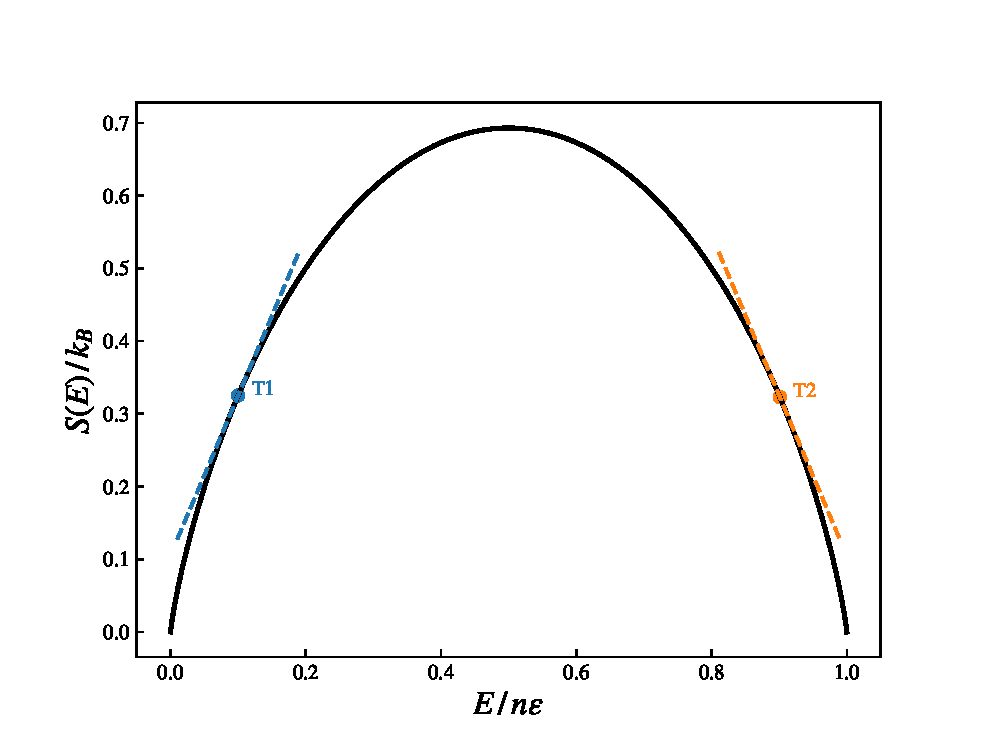
\includegraphics[scale=0.6]{./images/PandP_states.eps}
    \caption{The figure reports the relation between entropy and energy in a two levels system as found in chapter \ref{ch:TLS}. The system before the experiment was at equilibrium at a positive temperature $T_1$, while after the magnetic field inversion, the system 
    was found to be in an inverted population state described by a negative temperature $T_2$. The temperature is the reciprocal of the slope of the tangent of the plotted function in the two points.}
    \label{fig:PandP_switch}
\end{figure}
Experimentally it was known that the spins were aligned antiparallel with respect to the magnetic field by looking at the magnetic susceptibility of the system. To define such a quantity, let us first define the magnetization of the system as
\begin{equation}
    M = \sum_i M_i
\end{equation}
where $M_i$ is the projection of the magnetic moment vector $\ve M$ of the i-th particle along the magnetic field axis, or, in other words,
\begin{equation*}
    M_i = \mu \, S_i
\end{equation*}
where $S_i$ is the spin of the i-th particle. \\
The magnetic susceptibility $\chi$ is then defined as the constant such that
\begin{equation*}
    M = \chi \, H
\end{equation*}
A negative susceptibility then implies that the system is in an inverted population state, which means at negative temperatures. The scusceptibility as a function of time in the experiment is reported in figure \ref{fig:PandP_switch}, directly exported from the original article by Purcell and Pound \cite{PandP}.
\begin{figure}[htbp]
    \centering 
    \includegraphics[scale=0.5]{./images/PurcellPound.png}
    \caption{The plot (exported from \cite{PandP}) reports the record of the magnetic susceptibility during the experiment. The first peak denotes
    the initial equilibrium state in which the spins are aligned with the magnetic field in the lowest energy state. As the magnetic field is istantaneously reversed,
    the spins remained aligned in the opposite direction of the field, remaining in the highest enery state and causing the second (negative) peak. After a relaxation time
    $\tau_L$ the spin system returns at equilibrium in the lowest energy state.}
    \label{fig:PandP}
\end{figure}

\newpage

\section{Criticism against Boltzmann's entropy}
\label{sec:entropy}
\chapter{Issues on the definition of entropy}
\label{ch:entropy}
The definition of temperature via
\begin{equation*}
    \frac{1}{T} = \frac{\partial S(E)}{\partial E}
\end{equation*}
is strictly dependent on the definition of the entropy and the existence of negative temperatures is mainly a consequence of this definition. 
It was already discussed in chapter \ref{ch:temperature} why it is legitimate to define the temperature as the derivative of the entropy with respect to the energy. The purpose of this section, on the other side,
is to discuss the definition of the entropy with particular regards to the definitions given by Gibbs and Boltzmann since they have direct consequences on the existence of negative temperatures. \\
After a brief introduction over the two perspectives, the focus of the discussion will be on the comparison between the two definitions with particular emphasis on the direct consequences on the negative temperatures.

\section{Boltzmann's framework}
The conceptual basis for Boltzmann's approach to statistical mechanics presented in Boltzmann's paper (1877b) relies on the attempt to explain the Second Law of thermodynamics via probability calculus. \\
To introduce the idea let us consider a system of $N$ particles and let us work in a $6N$ dimensional phase space with coordinates $q_1,...,q_{3N}, p_1, ... p_{3N}$ and let us consider also the $\mu$-space associated to each particle in the system, i.e. the phase space in which each single particle moves. \\
Let us parition each $\mu$-space into $m$ disjoint rectangular cells of volume $\Delta\omega$ so that $\mu = \omega_1 \cup ... \cup \omega_m$ and each cell $\omega_i$ is charaterized by an energy value $\epsilon_i$. Once specifying the mechanical state of the system, a point $x \in \Gamma$, one can 
associate a collection of $N$ points in the $\mu$-spaces, one for each particle (the spaces are the same for each particle). For each $x$, also called \emph{microstate} of the system, one can define a \emph{macrostate} $Z$ for the system by specifying the number of particles $n_i$ included in each cell $\omega_i$ in the $\mu$-space. 
Formally $Z = (n_1, ... , n_m)$ where $n_i$ is the number of particles in the cell $\omega_i \subset \mu$. \\
By this definition it is clear that more than one microstate can describe the same macrostate of the system. One can associate a phase space volume to a macrostate $Z_0$, that is the set of corresponding microstates
\begin{equation*}
    \Gamma_{Z_0} \equiv \{x \in \Gamma : Z(x) = Z_0\}
\end{equation*}
The Boltzmann's entropy of a system in a macrostate $Z$ is then defined as
\begin{equation}
    S = k_B \ln\left( \text{Vol}(\Gamma_Z)\right)
    \label{eq:Boltzmann_entropy}
\end{equation}
In the case of a particle moving in the phase space, the microstates are counted by dividing the volume available for the particle in the phase space by the equivalent volume of one microstate, which, after quantum mechanics, it is known to be $h^3$.
In formulas, equation \ref{eq:Boltzmann_entropy} reduces to
\begin{equation*}
    S(E) = k_B \ln \omega(E)
\end{equation*}
where
\begin{equation*}
    \omega(E) = \frac{1}{h^3} \int \, d^3qd^3p \ \delta(E - H(q, p))
\end{equation*}
\section{Gibbs' framework}
Gibbs' approach to statistical mechanics is based on the idea of \emph{statistical ensemble}. To introduce this concept
let us work again in a phase space $\Gamma$ and describe the system via $3N$ canonical coordinates, so that $\Gamma$ is a $6N$ dimensional space. A point in $\Gamma$ denotes
a precise configuration of the system and it is referred to as a \emph{representative point}. \\
A given macroscopic configuration of the system can correspond to multiple microscopic configurations, that is multiple points in the $\Gamma$ space might correspond to the same macroscopic state. \\
In other words, when specifying a precise macroscopic configuration, we are not referring to one system, but rather to a collection of systems which we call an \emph{ensemble}. \\
An ensemble is conveniently described my means of a \emph{density function} $\rho(q, p ,t)$ such that $\rho(q, p, t) d^{3N}qd^{3N}p$ is the number of representative points in a phase space volume $d^{3N}qd^{3N}p$. \\
Given the value of $\rho$ at time $t=0$, the evolution of the function is completely determined by means of the Hamilton equation 
\begin{gather*}
    \frac{dp_i}{dt} = -\frac{\partial \mathcal H}{\partial q_i} \\
    \frac{dq_i}{dt} = \frac{\partial \mathcal H}{\partial p_i}
\end{gather*}
More precisely the evolution of $\rho$ is determined by the \emph{Liouville's theorem} which states that
\begin{equation}
    \frac{\partial \rho}{\partial t} + \sum_{i=1}^{3N} \left(\frac{\partial \rho}{\partial p_i}\dot p_i + \frac{\partial \rho}{\partial q_i} \dot q_i\right) = 0
\end{equation}
or 
\begin{equation*}
    \frac{\partial \rho}{\partial t} = \left\{H, \rho\right\}
\end{equation*}
\vspace{10pt}
In developing his theory, Gibbs' main goal was to produce a rational fundation for thermodynamics. Hence, Gibbs's work was guided by analogies between his theory and thermodynamics. \\
In his book \cite{gibbs_2010} Gibbs derived a relation in the canonical ensemble that is
\begin{equation}
    d\left\langle H \right\rangle = \theta d\sigma - \sum_i \left\langle A \right\rangle da_i
    \label{eq:fundamentaleq_Gibbs}
\end{equation}
which is formally analogue to the fundamental equation of thermodynamics
\begin{equation*}
    dU = TdS + \sum_i F_i da_i
\end{equation*}
where $\left\langle H \right\rangle$ in equation \ref{eq:fundamentaleq_Gibbs} denotes the expectation value of the hamiltonian in the canonical ensemble.
The analogy suggests that $\theta$, the so called \emph{modulus of the ensemble}, can be identified as the temperature of the system and  and $\sigma$, which was defined as
\begin{equation*}
    \sigma[\rho_{\theta}] = - \int \rho_{\theta}(x) \ln \rho_{\theta}(x) \, dx
\end{equation*}
can be identified as the entropy of the system, namely the \emph{Gibbs entropy}. \\
The important point is that, in the Gibbs' approach, the entropy is not a function on the phase space but rather a functional on the ensemble density $\rho_{\theta}$.
In principle one can propose a couple $(\theta, \sigma)$ arbitrarilly chosen and check if relation \ref{eq:fundamentaleq_Gibbs} is satisfied. \\
The next step is to understand whether an equation such \ref{eq:fundamentaleq_Gibbs} can be obtained in the microcanonical ensemble. Gibbs showed (see \cite{gibbs_2010} page 124-128, 169,171) that the relation is satisfied with the following definitions
\begin{gather*}
    T \quad \longleftrightarrow \quad \left(\frac{\partial \ln \Omega(E)}{\partial E}\right)^{-1} \\
    S \quad \longleftrightarrow \quad \ln \Omega(E)
\end{gather*}
where 
\begin{equation}
    \Omega(E) \equiv \int_{H(x) \leq E} \, dx
    \label{eq:Omega_E}
\end{equation}
is called \emph{integrated density of states}. 

\section{Consistent thermodynamics forbids negative temperatures}
The difference between the Gibbs entropy \footnote{the Boltzmann's constant is added for dimensional arguments}
\begin{equation}
    S_G = k_B \ln \Omega(E)
    \label{eq:gibbs_entropy_formula}
\end{equation}  
and the Boltzmann's entropy 
\begin{equation}
    S_B = k_B \ln \omega(E)
    \label{eq:Boltzmann_entropy_formula}
\end{equation}
has a direct and important consequence on the existence of negative temperatures. Indeed it is easy to see that the integrated density of states defined in equation 
\ref{eq:Omega_E}, that is the number of states whose energy is less than or equal to $E$, is a monotonically increasing function of the energy, hence the temperature is always positive. On the other side,
the density of states $\omega(E)$ that enters in the Boltzmann's entropy denotes the number of states in the range $(E, E+dE)$ and there is no reason to believe that is a monotonically increasing function of the energy. In fact we have already seen
that in the case of a non interacting two levels system the Boltmann's entropy leads to negative temperatures. \\
The choice of the correct microcanonical entropy is not a straightforward process since different definitions of the entropy can be used until they are able to reproduce thermodynamics. \\
In 1991 Berdichevsky \textit{et al.} \cite{original_entropy} pointed out some arguments in favour of Gibbs' entropy, which have then been developed by many authors. The main arguments were proposed by 
Dunkel and Hillbert in 2014 \cite{Dunkel_Hillbert} introducing the so called \emph{thermostatistical consistency condition}. \par 
\vspace{10pt} 
Let us suppose that the system is described by some control variables $\{E, V, A_i\}$ so that $S = S(E, V, A_i)$. By differentiating $S$ with respect to the control variables one obtains
\begin{equation*}
    \begin{aligned}
        \mathrm{d} S &=\left(\frac{\partial S}{\partial E}\right) \mathrm{d} E+\left(\frac{\partial S}{\partial V}\right) \mathrm{d} V+\sum_{i}\left(\frac{\partial S}{\partial A_{i}}\right) \mathrm{d} A_{i} \\
        & \equiv \frac{1}{T} \mathrm{~d} E+\frac{p}{T} \mathrm{~d} V+\sum_{i} \frac{a_{i}}{T} \mathrm{~d} A_{i}
        \end{aligned}
\end{equation*}
If one now considers an isoentropic process for which only energy and one control variable are allowed to change, one gets that
\begin{equation}
    T\left(\frac{\partial S}{\partial A_{\mu}}\right)_{E}=-\left(\frac{\partial E}{\partial A_{\mu}}\right)_{S}=-\left\langle\frac{\partial H}{\partial A_{\mu}}\right\rangle
    \label{eq:cond1}
\end{equation}
Now, since
\begin{equation}
    \begin{array}{l}
        T_{\mathrm{B}}(E, V, A)=\left(\frac{\partial S_{\mathrm{B}}}{\partial E}\right)^{-1} = \frac{1}{k_{\mathrm{B}}} \frac{\Omega^{\prime}}{\Omega^{\prime \prime}} \\
        T_{\mathrm{G}}(E, V, A)=\left(\frac{\partial S_{\mathrm{G}}}{\partial E}\right)^{-1}=\frac{1}{k_{\mathrm{B}}} \frac{\Omega}{\Omega'}
        \end{array}
    \label{eq:temperatures_definition}
\end{equation}
where the prime indicates the differentiation with respect to the energy of the system, one has that 
\begin{gather*}
    T_B \left(\frac{\partial S_B}{\partial A_{\mu}}\right) = \frac{1}{\Omega''} \frac{\partial \Omega'}{\partial A_{\mu}} \\
    T_G \left(\frac{\partial S_G}{\partial A_{\mu}}\right) = \frac{1}{\Omega'} \frac{\partial \Omega}{\partial A_{\mu}}
\end{gather*}
so in general we expect that if one of the two definitions of entropy satisfies condition \ref{eq:cond1}, the other one does not, and it is easy to see that the Gibbs' entropy does
\begin{equation*}\begin{aligned}
    T_{G}\left(\frac{\partial S_{G}}{\partial A_{\mu}}\right) &=\left(\frac{\partial S_{G}}{\partial E}\right)^{-1}\left(\frac{\partial S_{G}}{\partial A_{\mu}}\right)=\frac{1}{\omega} \frac{\partial}{\partial A_{\mu}} \int \, dx \ \theta(E-\mathcal{H}(x)) \\
    &=\frac{1}{\omega} \int \, dx \ \frac{\partial \theta(E-\mathcal{H}(x))}{\partial A_{\mu}} = -\frac{1}{\omega} \int \, dx \ \delta(E-\mathcal{H}(x)) \frac{\partial \mathcal{H}(x)}{\partial A_{\mu}} \\
    &=-\int \, dx \ \frac{\delta(E-\mathcal{H})}{\omega} \frac{\partial \mathcal{H}}{\partial A_{\mu}} = -\int \, dx \ \rho \frac{\partial \mathcal{H}}{\partial A_{\mu}} = -\left\langle\frac{\partial \mathcal{H}}{\partial A_{\mu}}\right\rangle
\end{aligned}\end{equation*}
Another argument in favour of Gibbs' entropy, still proposed by Dunkel and Hillbert \cite{Dunkel_Hillbert}, is that it satisfies the generalized equipartition theorem
\begin{equation}
    \left\langle\xi_{i} \frac{\partial \mathcal{H}}{\partial \xi_{j}}\right\rangle=\delta_{i j} T
    \label{eq:equipartition}
\end{equation}
while Boltzmann's does not.  \\
To see this one can consider the simple example of an ideal gas confined in a cubic box of side $L$. In this case the hamiltonian reads 
\begin{equation*}
    \mathcal{H}(t,\ve q,\ve p) = \sum_i \frac{\ve{p}_i^2}{2m} + V(\ve q_i)
\end{equation*}
where 
\begin{equation*}
    V(\ve{q}_i) = 
    \begin{cases}
        0 \qquad \text{if } \ve q_i \in \text{box} \\
        +\infty \qquad \text{otherwise}
    \end{cases}
\end{equation*}
The integrated density of states, that is the number of states with energy less than or equal to $E$, can be computed as 
\begin{gather*}
    \Omega(E) = \frac{1}{h^{3N}} \, \int d^{3N}p \int d^{3N}q \quad \theta(E-\mathcal{H}(t, \ve q, \ve p)) = \\ = \frac{V^N}{h^{3N}} \, \int d^{3N}p \quad \theta\left(E - \sum_i \frac{\ve{p}_i^2}{2m}\right) 
    = \frac{V^N \, (2\pi mE)^{3N/2}}{h^{3N} \, \Gamma(\frac{3N}{2}+1)}
\end{gather*}
so that the density of states is 
\begin{gather*}
    \omega(E)=\frac{\partial \Omega}{\partial E}=\frac{3 N V^{N}(2 \pi m)^{3 N / 2}}{2 h^{3} \Gamma\left(\frac{3 N}{2}+1\right)} E^{\frac{3 N}{2}-1}
\end{gather*}
One can now calculate the two temperatures using \ref{eq:temperatures_definition}
\begin{gather*}
    \frac{1}{T_{G}}=\frac{\partial S_{G}}{\partial E}=\frac{\partial \ln \Omega}{\partial E}=\frac{h^{3} \Gamma\left(\frac{3 N}{2}+1\right)}{V^{N}(2 \pi m E)^{3 N / 2}} \frac{3 N V^{N}(2 \pi m)^{3 N / 2}}{2 h^{3} \Gamma\left(\frac{3 N}{2}+1\right)} E^{\frac{3 N}{2}-1} \\
    \frac{1}{T_{B}}=\frac{\partial S_{B}}{\partial E}=\frac{\partial \ln \omega}{\partial E}=\left(\frac{3 N V^{N}(2 \pi m)^{3 N / 2}}{2 h^{3} \Gamma\left(\frac{3 N}{2}+1\right)} E^{\frac{3 N}{2}-1}\right)^{-1} \frac{3 N}{2}\left(\frac{3 N}{2}-1\right) E^{\frac{3 N}{2}-2}
\end{gather*}
and rearranging terms 
\begin{equation}\begin{gathered}
    E=\frac{3 N}{2} T_{G} \\
    E=\left(\frac{3 N}{2}-1\right) T_{B}
\end{gathered}
\label{eq:equipartition_results}
\end{equation}
showing that only the Gibbs' entropy satisfies the equipartition theorem. \par
\vspace{10pt}
The fact that Gibbs' entropy was "the correct entropy" created some disturb. This was mainly because of the unphysical meaning of Gibbs' entropy. Why should one 
take into account the states with a different energy of the system when calculating the number of microstates available for a given energy $E$? \\
Another position on the issue was indeed argued by Frenkel and Warren \cite{Frenkel} who not only showed that Boltzmann's entropy satisfies the thermodynamic condition in the thermodynamic limit, but also that Gibbs' entropy fails to meet a basic thermodynamic criterion which is 
the equality of the temperatures of two systems in reciprocal equilibrium. \\
Let us consider a two level system $\mathcal{S}_1$ with bounded phase space (e.g. a two levels system) in an inverted population state. According to what seen in chapter \ref{ch:TLS}, the system is described by a negative temperature, say $T_{1,B}$, using the Boltzmann's definition. Instead if one makes use of the Gibbs' definition of temperature, the latter is certainly positive since $T_G$ does not admit negative values: let us call this value $T_{1,G}$. \\
It is then possible to create another system $\mathcal{S}_2$ with an unbounded phase space, for example a free ideal gas, such that $T_{2,G} = T_{1,G}$, but obviously $T_{2,B} \neq T_{1,B}$, since the free ideal gas does not admit negative Boltzmann temperature. According to what told in chapter \ref{ch:temperature}, $T_{2,G} = T_{1,G}$ implies that the two systems are in equilibrium, while $T_{2,B} \neq T_{1,B}$ predicts them to be out of equilibrium. 
When the two systems are put into contact, they are allowed to exchange heat keeping the total energy of the collective system constant. The configuration that is most probable at equilibrium is the one that maximizes the entropy of the whole system compatibly with the available energy. \\
Since the system $\mathcal{S}_1$ is not in its maximum entropy state, when allowed to exchange heat to $\mathcal{S}_2$, it lowers its energy releasing heat increasing also $\mathcal{S}_2$'s entropy.
This means that $\mathcal{S}_1$ and $\mathcal{S}_2$ were out of equilibrium implying Gibbs's temperature to be wrong. \par
\vspace{10pt}
The only issue that needs to be solved now is to understand why Boltzmann's entropy does not satisfy the thermodynamic consistency relation or the equipartition theorem as previously shown. Frenkel and Warren argued that the conditions are instead satisfied also by the Boltzmann's definition of entropy in the thermodynamic limit, that is for $N \gg 1$, that is the limit in which statistical mechanics is expected to connect to thermodynamics.
This is obvious for the particular case of the ideal gas which leads to \ref{eq:equipartition_results} and it is immediate to check that the two expressions coincide in the limit of large $N$. \\
To prove that the consistency relation is respected in the general case, let us first start by proving that, in the canonical ensemble, the following relation holds
\begin{equation}
    -\left.\frac{\partial F}{\partial A_{\mu}}\right|_{T}=-\left\langle\frac{\partial H}{\partial A_{\mu}}\right\rangle_{T}
    \label{eq:entropy_eq_1}
\end{equation}
Since $F = -\frac{1}{\beta} \ln Z$, where
\begin{equation*}
    Z = \sum_x e^{-\beta H(x)}
\end{equation*} 
then 
\begin{equation}
    e^{-\beta F}=\sum_x e^{-\beta H(x)}
    \label{eq:free_energy_rel1}
\end{equation}
Differentiating both members with respect to $A_{\mu}$ gives 
\begin{equation}
    -\left.\beta \frac{\partial F}{\partial A_{\mu}}\right|_{T} e^{-\beta F}=-\beta \sum \frac{\partial H}{\partial A_{\mu}} e^{-\beta H}
    \label{eq:free_energy_rel2}
\end{equation}
and by taking the ratio of equations \ref{eq:free_energy_rel1} and \ref{eq:free_energy_rel2}, the result is proved. \\
Now, to prove the consistency relation \ref{eq:cond1}, we need to move to the microcanonical ensemble. In this case the averages are performed as 
\begin{equation*}
    \langle\cdots\rangle_{E}=\frac{\int (\cdots) \delta(E-H)}{\int \delta(E-H)}
\end{equation*}
and the equivalent of \ref{eq:free_energy_rel1} for the entropy is
\begin{equation*}
    \int \delta(E-H) = e^{S_{\mathrm{B}} / k_{\mathrm{B}}}
\end{equation*}
One can write that
\begin{gather*}
    \int \, dx \ (...) \ e^{-\beta H(x)} = \int \, dE \int \, dx \ (...) \ \delta(E-H(x)) \, e^{-\beta E} =  \\
    = \int \, dE \ e^{-\beta E} \int \, dx \ (...) \ \delta(E-H(x))
\end{gather*}
Let us multiply and divide the left member by $Z = e^{-\beta F}$ and the right member by $e^{-\beta E + S_B/k_B}$ obtaining
\begin{equation}
    e^{-\beta F}\langle\cdots\rangle_{T}=\int_{0}^{\infty} d E e^{-\beta E+S_{\mathrm{B}} / k_{\mathrm{B}}}\langle\cdots\rangle_{E}
    \label{eq:entropy_eq_2}
\end{equation}
where $\langle\cdots\rangle_{T}$ and $\langle\cdots\rangle_{E}$ indicate the averages in the canonical and microcanonical ensemble respectively. The last equation, in the special case of $(...) = 1$ yields
\begin{equation*}
    e^{-\beta F} = \int e^{-\beta E+S_{\mathrm{B}} / k_{\mathrm{B}}}
\end{equation*}
Now, the last integral is peaked around a value $E^*$ and the higher the number of degrees of freedom in the system, the more peaked the integrand. In the
thermodynamic limit, let us then evaluate this last integral by the saddle point method. We obtain that 
\begin{equation*}
    -\beta F=-\beta E+\frac{S_{\mathrm{B}}}{k_{\mathrm{B}}}
\end{equation*}
where $-\beta+\frac{\partial}{\partial E}\left(\frac{S_{\mathrm{B}}}{k_{\mathrm{B}}}\right)=0$ (condition for the extremum). Recalling that $\beta=\frac{1}{k_BT}$, the condition for the extremum states that 
$\frac{1}{T} = \frac{\partial S_B}{\partial E} = \frac{1}{T_B}$. Hence
\begin{equation}
    F = E - TS
    \label{eq:free_energy_def}
\end{equation}
where $T = T_B = \frac{\partial S_B}{\partial E}$ which is the definition of the Legendre transform of the energy with respect to the couple $T \leftrightarrow S$. \\
In an analogous way it is possible to apply the same method to \ref{eq:entropy_eq_2} obtaining as a result that 
\begin{equation}
    \langle\cdots\rangle_{T} = \langle\cdots\rangle_{E}
    \label{eq:equivalence_of_averages}
\end{equation}
Now, by differentiating equation \ref{eq:free_energy_def} with respect to $A_{\mu}$, one gets that
\begin{equation*}
    \left.\frac{\partial F}{\partial A_{\mu}}\right|_{T}=\left(1-T \frac{\partial S_{\mathrm{B}}}{\partial E}\right) \frac{\partial E}{\partial A_{\mu}}-\left.T \frac{\partial S_{\mathrm{B}}}{\partial A_{\mu}}\right|_{E} = -\left.T \frac{\partial S_{\mathrm{B}}}{\partial A_{\mu}}\right|_{E}
\end{equation*}
combining this result with \ref{eq:entropy_eq_1}, \ref{eq:equivalence_of_averages} and the fact that $T = T_B = \frac{\partial S}{\partial E}$, we get the desired result
\begin{equation*}
    \left.T_{\mathrm{B}} \frac{\partial S_{\mathrm{B}}}{\partial A_{\mu}}\right|_{E}=-\left\langle\frac{\partial H}{\partial A_{\mu}}\right\rangle_{E}
\end{equation*}

\newpage

\printbibliography
\end{document}